\chapter{植物如何传播}\label{ch:g6:how-plants-spread}

三月，一段新修的道路切坡被推土机推平：裸露的生土，
看不到一点绿色。到九月再来看，这里已密密麻麻
长满\omterm{prop:g2:from-seed-to-plant:cycle}{幼苗}——罂粟、蒲公英、柳树苗、禾草。没有人播种。然而\omterm{def:g1:plants-around-us:plant}{植物}
并不能迈出一步，却在短短几个月内就\omterm{prop:g6:how-plants-spread:travel}{定殖}了这片裸地。
本章讲的是它们的
“旅行部门”。

\section{植物借种子和孢子远行}

\begin{proposition}[定居的植物，外出的繁殖体]\label{prop:g6:how-plants-spread:travel}
成年\omterm{def:g1:plants-around-us:plant}{植物}一生固定不动
（见\cref{def:g1:plants-around-us:plant}）——因此一个\omterm{def:g5:biodiversity:species}{物种}
通过送出自己的\emph{繁殖体}：\omterm{def:g2:from-seed-to-plant:seed}{种子}和
\omterm{prop:g3:flowers-fruits-seeds:transform}{果实}（见\cref{ch:g5:flower-to-fruit}）、\omterm{def:g4:plants-without-seeds:spore}{孢子}
（见\cref{def:g4:plants-without-seeds:spore}）、\omterm{ex:g4:plants-without-seeds:runner}{匍匐茎}和
其他\omterm{def:g4:plants-without-seeds:vegetative}{营养繁殖}结构
（见\cref{def:g4:plants-without-seeds:vegetative}）。以这种方式占据
新的土地，称为
\emph{定殖}\index{定殖}。
\end{proposition}
\admitted

\begin{definition}[扩散]\label{def:g6:how-plants-spread:dispersal}
\emph{扩散}\index{扩散}是指\omterm{def:g2:from-seed-to-plant:seed}{种子}、
\omterm{prop:g3:flowers-fruits-seeds:transform}{果实}或\omterm{def:g4:plants-without-seeds:spore}{孢子}离开母株的过程。搬运者
很少，而且历史悠久：\emph{风}、\emph{\omterm{def:g1:animals-around-us:animal}{动物}}、
\emph{水}——还有一些\omterm{prop:g3:flowers-fruits-seeds:transform}{果实}会靠自身
把\omterm{def:g2:from-seed-to-plant:seed}{种子}弹射出去。
\end{definition}

\begin{example}[为什么要离开家？]\label{ex:g6:how-plants-spread:whyleave}
\omterm{def:g2:from-seed-to-plant:seed}{种子}若落在母株脚下，就在母株的树荫里\omterm{def:g2:from-seed-to-plant:germination}{萌发}，
与母株的根挤在一起，争夺的正是
光与水（见\cref{prop:g4:what-plants-need:needs}），
对手的体形却是它的一百倍。
\omterm{def:g6:how-plants-spread:dispersal}{扩散}正是摆脱这场
注定落败的竞争的办法：距离
是\omterm{def:g1:plants-around-us:plant}{植物}送给幼体的第一份礼物。
\end{example}

\section{搬运者，以及为它们而生的果实}

\begin{proposition}[果实与搬运者相匹配]\label{prop:g6:how-plants-spread:builds}
\omterm{prop:g3:flowers-fruits-seeds:transform}{果实}与\omterm{def:g2:from-seed-to-plant:seed}{种子}的形态与搬运者相匹配——
即\cref{def:g4:adapted-to-their-world:adaptation}中“\omterm{def:g4:adapted-to-their-world:adaptation}{适应}”的概念，
只是用在“行李”上：
\begin{itemize}
  \item \emph{风}：降落伞（蒲公英的\omterm{def:g1:animals-around-us:covering}{羽毛}状
        \omterm{def:g2:from-seed-to-plant:seed}{种子}）、翅膀（槭树和白蜡树的翅果，斜着旋转而下）、
        或细如微尘、只靠漂浮的\omterm{def:g4:plants-without-seeds:spore}{孢子}
        （\omterm{prop:g4:plants-without-seeds:damp}{蕨类}的\omterm{def:g4:plants-without-seeds:spore}{孢子}数以百万计）；
  \item \emph{\omterm{def:g1:animals-around-us:animal}{动物}，体外}：带钩的\omterm{prop:g3:flowers-fruits-seeds:transform}{果实}——牛蒡、
        猪殃殃——它们的钩子钩住\omterm{def:g1:animals-around-us:covering}{皮毛}和袜子，随之一路
        直到被梳理掉；
  \item \emph{\omterm{def:g1:animals-around-us:animal}{动物}，体内}：多汁的肉质\omterm{prop:g3:flowers-fruits-seeds:transform}{果实}——
        樱桃、黑莓、蔷薇果——整个被吃下；
        种皮坚硬的\omterm{def:g2:from-seed-to-plant:seed}{种子}完好地通过\omterm{def:g4:journey-of-food:tract}{消化道}，
        随粪便被排到别处，并带着肥料
        （见\cref{exo:g3:flowers-fruits-seeds:10}的解答，
        已补充完整）；
  \item \emph{水}：漂浮的\omterm{prop:g3:flowers-fruits-seeds:transform}{果实}——桤木的小
        木筏、椰子那能漂洋过海的硬壳；
  \item \emph{自行弹射}：干燥后会绷紧并猛然开裂的荚果
        ——金雀花和堇菜能把\omterm{def:g2:from-seed-to-plant:seed}{种子}弹出，
        离母株数米远。
\end{itemize}
\end{proposition}
\admitted

\begin{omfigure}
\begin{tikzpicture}[scale=0.9]
  % dandelion parachute
  \draw[very thick, omExo!80] (0.7,0.3) -- (0.7,1.2);
  \foreach \a in {50,70,90,110,130} {
    \draw[omExo] (0.7,1.2) -- ++(\a:0.55);
  }
  \fill[omExo] (0.7,0.3) ellipse (0.06 and 0.14);
  \node[font=\small, align=center] at (0.7,-0.55)
    {降落伞：\\ 风};
  % maple key
  \begin{scope}[xshift=3.5cm]
    \fill[omProp!50] (0.3,0.65) ellipse (0.14 and 0.2);
    \draw[thick, omProp!80!black, fill=omProp!15]
      (0.38,0.78) .. controls (0.9,1.5) and (1.6,1.35) .. (1.75,0.95)
      .. controls (1.3,1.05) and (0.7,0.8) .. (0.42,0.6);
    \node[font=\small, align=center] at (0.95,-0.55)
      {旋转翅果：\\ 风};
  \end{scope}
  % burr
  \begin{scope}[xshift=7.2cm]
    \draw[thick, fill=omMeth!15] (0.7,0.8) circle (0.3);
    \foreach \a in {0,30,...,330} {
      \draw[thick, omMeth!70!black] (0.7,0.8) ++(\a:0.3) -- ++(\a:0.22)
        ++(\a:0.0) -- ++({\a+120}:0.1);
    }
    \node[font=\small, align=center] at (0.7,-0.55)
      {带钩的果实：\\ 皮毛与袜子};
  \end{scope}
  % berry
  \begin{scope}[xshift=11.2cm]
    \draw[thick, fill=omThm!25] (0.7,0.8) circle (0.32);
    \fill[omThm!60!black] (0.62,0.82) circle (0.05);
    \fill[omThm!60!black] (0.8,0.72) circle (0.05);
    \draw[thick, omMeth!80!black] (0.7,1.12) -- (0.78,1.38);
    \node[font=\small, align=center] at (0.7,-0.55)
      {多汁的浆果：被吃掉，\\ 种子在体内随行};
  \end{scope}
\end{tikzpicture}

{\small 四件旅行装备。把每个形状都当作一张
地址标签来读：它标明传播者。}
\end{omfigure}

\begin{omfigure}
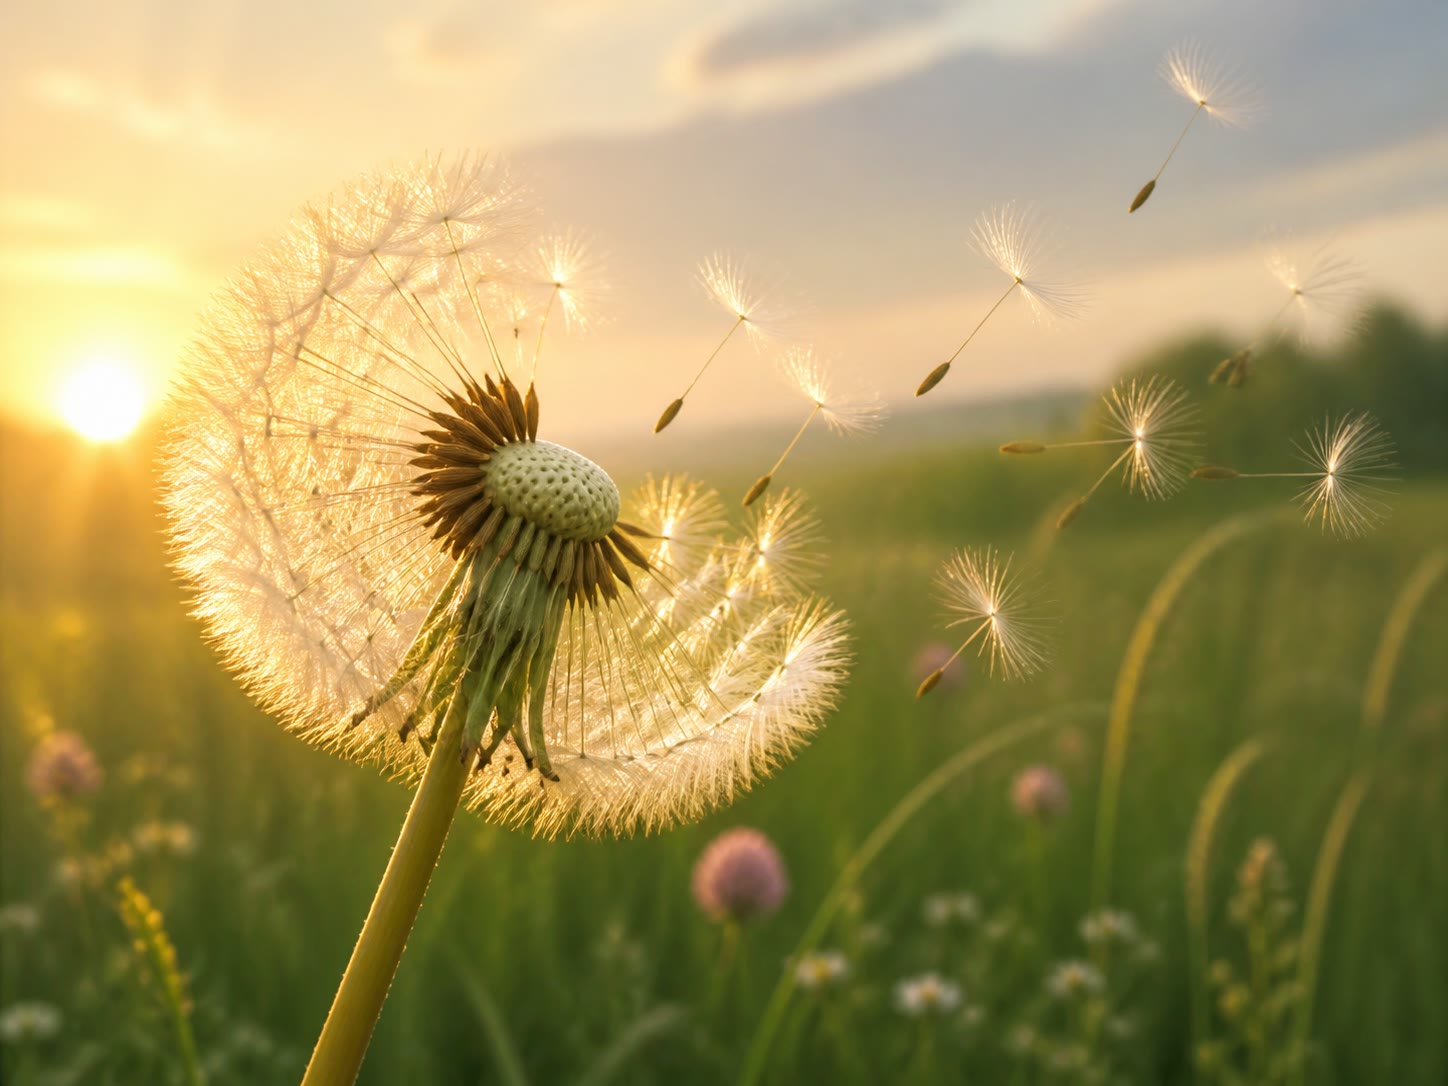
\includegraphics[width=0.58\linewidth]{images/book1/ai/g6-spread-dandelion.jpg}

{\small 风力运送服务正在进行中：每粒带冠毛的\omterm{def:g2:from-seed-to-plant:seed}{种子}都是
一次性的远距离旅行者。}
\end{omfigure}

\begin{example}[读懂路边的景象]\label{ex:g6:how-plants-spread:roadside}
九月路堑的解读：蒲公英和柳树——
带冠毛的\omterm{def:g2:from-seed-to-plant:seed}{种子}，借风飘来；罂粟——它们的细小
\omterm{def:g2:from-seed-to-plant:seed}{种子}早已躺在翻动过的土里，静候着，只有\omterm{def:g2:from-seed-to-plant:seed}{种子}才有这样的耐心
（见\cref{exo:g2:from-seed-to-plant:9}）；黑莓
\omterm{prop:g2:from-seed-to-plant:cycle}{幼苗}长在篱笆桩底下——由停歇的鸟儿带来，
连同肥料一起；路边的牛蒡——由
狗带进来。每个\omterm{prop:g6:how-plants-spread:travel}{定殖}者的抵达路线，都写在它的
装备之中。
\end{example}

\begin{method}[从果实判断传播者]\label{met:g6:how-plants-spread:name}
给定一个\omterm{prop:g3:flowers-fruits-seeds:transform}{果实}或\omterm{def:g2:from-seed-to-plant:seed}{种子}：
\begin{enumerate}
  \item 寻找飞行装置——冠毛、翅膀，或
        细如尘埃：由风传播；
  \item 寻找钩刺：\omterm{def:g1:animals-around-us:animal}{动物}\omterm{def:g1:animals-around-us:covering}{皮毛}，体外附着；
  \item 肉质、有颜色、味甜？\omterm{def:g1:animals-around-us:animal}{动物}肠道，体内——
        检查\omterm{def:g2:from-seed-to-plant:seed}{种子}是否有坚硬的种皮；
  \item 能浮水，靠近水边？水力传播；
  \item 干燥、扭曲、有弹性的荚果？自身弹射；
  \item 检验判断：让它下落，让它漂浮，把它
        贴到一只毛茸茸的袖子上。
\end{enumerate}
\end{method}

\section{不靠种子的定殖}

\begin{example}[地面上的推进]\label{ex:g6:how-plants-spread:vegetative}
与随风而来的\omterm{prop:g6:how-plants-spread:travel}{定殖}者并行，还有一些\omterm{prop:g6:how-plants-spread:travel}{定殖}者靠自己的
营养器官行走
（见\cref{ch:g4:plants-without-seeds}）：偃麦草借
\omterm{ex:g4:plants-without-seeds:runner}{匍匐茎}在地下推进，一米一米地前进；黑莓的枝条
弯向地面，尖端触地处生根；草莓的\omterm{ex:g4:plants-without-seeds:runner}{匍匐茎}
在空地上跳跃前进。慢，距离近——而且
在无人照管的花园里势不可挡，任何园丁都深知
这一点。
\end{example}

\begin{remark}[双速定殖]\label{rem:g6:how-plants-spread:twospeeds}
两套系统分工合作。\omterm{def:g2:from-seed-to-plant:seed}{种子}和\omterm{def:g4:plants-without-seeds:spore}{孢子}承担的是
\emph{远距离}服务——少数幸运的降落，远在他处，
比如蒲公英飞过小镇。营养推进则承担的是
\emph{近距离}服务——密集而稳妥地占据
近邻的土地。从树篱蔓延开来的黑莓丛同时使用两种方式：
弯曲的枝条负责一米之内，\omterm{prop:g3:sorting-living-things:groups}{鸟类}带来的\omterm{def:g2:from-seed-to-plant:seed}{种子}负责
数英里之外。
\end{remark}

\section{练习}

\begin{exercise}[$\star$]\label{exo:g6:how-plants-spread:1}
什么是\omterm{prop:g6:how-plants-spread:travel}{定殖}？什么是\omterm{def:g6:how-plants-spread:dispersal}{扩散}，
主要的传播者有哪些？
\end{exercise}

\begin{exercise}[$\star$]\label{exo:g6:how-plants-spread:2}
为什么\omterm{def:g2:from-seed-to-plant:seed}{种子}远离亲株\omterm{def:g2:from-seed-to-plant:germination}{萌发}更有利？
\end{exercise}

\begin{exercise}[$\star$]\label{exo:g6:how-plants-spread:3}
说出下列各项的传播者：蒲公英的冠毛、
牛蒡的钩刺果、樱桃、枫树的翅果、椰子。
\end{exercise}

\begin{exercise}[$\star$]\label{exo:g6:how-plants-spread:4}
被鸟吃掉的黑莓\omterm{def:g2:from-seed-to-plant:seed}{种子}如何度过这段旅程，
它们到达时带着什么？
\end{exercise}

\begin{exercise}[$\star$]\label{exo:g6:how-plants-spread:5}
荆豆和紫罗兰使用哪一种运送服务？描述
其机制。
\end{exercise}

\begin{exercise}[$\star$]\label{exo:g6:how-plants-spread:6}
举出两种营养\omterm{prop:g6:how-plants-spread:travel}{定殖}者，并说明各自如何推进。
\end{exercise}

\begin{exercise}[$\star\star$]\label{exo:g6:how-plants-spread:7}
解读路堑：对蒲公英、罂粟、黑莓
和牛蒡，给出本章所述的抵达路线。
\end{exercise}

\begin{exercise}[$\star\star$]\label{exo:g6:how-plants-spread:8}
依据\cref{met:g6:how-plants-spread:name}判断：（a）带冠毛的
蓟\omterm{def:g2:from-seed-to-plant:seed}{种子}；（b）蔷薇果；（c）一个粘在你套头衫上的
猪殃殃果球。
\end{exercise}

\begin{exercise}[$\star\star$]\label{exo:g6:how-plants-spread:9}
结合\cref{rem:g6:how-plants-spread:twospeeds}中的
“双速”思想，以黑莓丛为例加以解释：哪一套系统
负责一米之内，哪一套负责数英里之外？
\end{exercise}

\begin{exercise}[$\star\star$]\label{exo:g6:how-plants-spread:10}
\omterm{prop:g4:plants-without-seeds:damp}{蕨类}\omterm{prop:g6:how-plants-spread:travel}{定殖}了新插条潮湿的北岸，
却未能\omterm{prop:g6:how-plants-spread:travel}{定殖}其干燥的南岸。综合
\cref{prop:g4:plants-without-seeds:damp}和
\cref{prop:g6:exploring-our-environment:decide}，给出
该现象的解释。
\end{exercise}

\begin{exercise}[$\star\star$]\label{exo:g6:how-plants-spread:11}
一座岛屿从海中拔起，光秃秃的，距岸数公里。
哪些传播方式能够到达它？预测
其最初\omterm{def:g1:plants-around-us:plant}{植物}拓殖者的“装备”。
\end{exercise}

\begin{exercise}[$\star\star\star$]\label{exo:g6:how-plants-spread:12}
甜美的果肉对\omterm{def:g1:plants-around-us:plant}{植物}来说造价不菲。利用
\cref{ex:g6:how-plants-spread:whyleave}以及
\omterm{def:g1:animals-around-us:animal}{动物}体内传播的方式，解释樱桃树用这些糖分
换来了什么——并说明
\omterm{def:g2:from-seed-to-plant:seed}{种子}坚硬的外皮为何是这笔交易的另一半。
\end{exercise}

\section{问题：被弃置的田地}

\begin{problem}[{周末问题——十年的
拓殖，从一扇门观察}]\label{pb:g6:how-plants-spread:1}
一块耕过的田地在秋季被弃置。一位博物学家
每年六月都从门口为它拍照，连续十年，并
做记录。

\medskip\noindent\textbf{第一部分——第一年。}
\begin{enumerate}
  \item 第一年六月：裸露的土地上散布着
        罂粟、蒲公英和蓟。对每一种\omterm{def:g1:plants-around-us:plant}{植物}，说出
        其可能的来源与途径：罂粟来自
        土壤本身，其余的借风传播。是什么“装备”
        使借风到达者成为可能？
  \item 第一年田地中央没有黑莓出现，
        但旧篱笆桩下站着三株\omterm{prop:g2:from-seed-to-plant:cycle}{幼苗}。
        用\omterm{def:g1:animals-around-us:animal}{动物}体内传播的方式解释这一格局——
        为什么恰好在
        桩下？
  \item 博物学家在任何地方都找不到\omterm{prop:g4:plants-without-seeds:damp}{蕨类}，尽管
        逆风方向有一片满是\omterm{prop:g4:plants-without-seeds:damp}{蕨类}的林地。\omterm{prop:g4:plants-without-seeds:damp}{蕨类}的\omterm{def:g4:plants-without-seeds:spore}{孢子}
        肯定已经到达（\cref{ex:g4:plants-without-seeds:fern}
        统计了其数以百万计的数量）。根据
        \cref{prop:g4:plants-without-seeds:damp}，开阔田地的什么\omterm{def:g6:exploring-our-environment:conditions}{条件}
        拒绝了它们？
  \item 偃麦草只从田地边缘入侵，每年
        仅前进一米或两米。这是哪一种拓殖方式，
        为什么它不能像蒲公英那样
        出现在田地中央？
\end{enumerate}

\medskip\noindent\textbf{第二部分——之后的岁月。}
\begin{enumerate}[resume]
  \item 到第三年，禾草和高大草本已覆盖
        裸露的地面，罂粟已从
        现存植被中消失。罂粟如今在哪里，
        以什么形式存在？（回想道路切坡以及
        \cref{prop:g6:life-through-seasons:herbs}。）
  \item 从第四年起，黑莓弯枝与幼小的山楂
        散布于田地各处，在树篱附近和
        篱笆线下最为密集。说出放置它们的
        两种传播方式，并指出格局中的证据。
  \item 到第八年，柳树和桦树幼树已
        高过黑莓——两者都有细小的
        带\omterm{def:g1:animals-around-us:covering}{羽毛}或轻如尘埃的\omterm{def:g2:from-seed-to-plant:seed}{种子}。为什么\omterm{def:g2:from-seed-to-plant:seed}{种子}沉重的
        橡树和栗树仍几乎不见踪影？最终
        又是哪种\omterm{def:g1:animals-around-us:animal}{动物}信使把它们也种了下来？
  \item 照片显示，田地的植被构成
        逐年变化，尽管无人照料。请陈述
        其背后的驱动规律：每年的植被
        如何改变田地自身的\omterm{def:g6:exploring-our-environment:conditions}{条件}——
        尤其是地面高度的光照，并说明这一改变
        有利于谁成为下一个受益者？
\end{enumerate}

\medskip\noindent\textbf{第三部分——总体启示。}
\begin{enumerate}[resume]
  \item 按到达先后排列拓殖者：土壤中等待的
        \omterm{def:g2:from-seed-to-plant:seed}{种子}、借风飞行的\omterm{def:g1:plants-around-us:plant}{植物}、由\omterm{def:g1:animals-around-us:animal}{动物}携带的灌木、
        \omterm{def:g2:from-seed-to-plant:seed}{种子}沉重的乔木。将每一批拓殖者与
        使其到达时间得以确定的传播方式一一对应。
  \item 城镇广场人行道的裂缝中会长出相同的
        第一年\omterm{def:g1:plants-around-us:plant}{植物}群——罂粟、蒲公英——但
        永远长不到第四年的灌木。给出该演替
        在此停滞的两个理由。
  \item 博物学家断言：“若任其自然，这片田地
        将变成林地。”请用
        十年变化趋势为这一论断辩护，并指出
        \cref{prop:g5:people-and-nature:managed}中的草甸例外，
        说明“任其自然”才是关键用语。
  \item 用两句话概括整个问题，并使用
        \emph{传播}、\emph{\omterm{def:g6:exploring-our-environment:conditions}{条件}}和
        \emph{拓殖}。
\end{enumerate}
\end{problem}
